\documentclass{article}
\usepackage{tikz}
\usetikzlibrary{arrows.meta}

\begin{document}

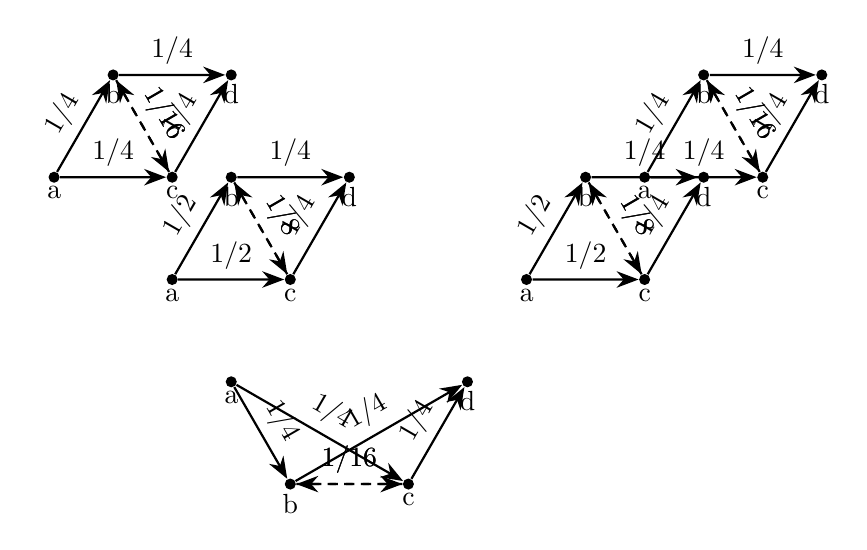
\begin{tikzpicture}[scale=1.5]
    % Define styles for nodes and edges
    \tikzstyle{vertex}=[circle,fill=black,minimum size=4pt,inner sep=0pt]
    \tikzstyle{edge} = [draw,thick,-{Stealth[scale=1.2]}]

    % Draw the first part of the tree
    \node[vertex] (a) at (-1,0) {};
    \node[vertex] (b) at (-0.5,-0.866) {};
    \node[vertex] (c) at (0.5,-0.866) {};
    \node[vertex] (d) at (1,0) {};

    \draw[edge] (a) -- node[above,sloped] {$1/4$} (b);
    \draw[edge] (a) -- node[above,sloped] {$1/4$} (c);
    \draw[edge] (b) -- node[above,sloped] {$1/4$} (d);
    \draw[edge] (c) -- node[above,sloped] {$1/4$} (d);

    \draw[edge,dashed] (b) -- node[above,sloped] {$1/16$} (c);
    \draw[edge,dashed] (c) -- node[above,sloped] {$1/16$} (b);

    \node[vertex] (a1) at (-1.5,0.866) {};
    \node[vertex] (b1) at (-1,1.732) {};
    \node[vertex] (c1) at (-0.5,0.866) {};
    \node[vertex] (d1) at (0,1.732) {};

    \draw[edge] (a1) -- node[above,sloped] {$1/2$} (b1);
    \draw[edge] (a1) -- node[above,sloped] {$1/2$} (c1);
    \draw[edge] (b1) -- node[above,sloped] {$1/4$} (d1);
    \draw[edge] (c1) -- node[above,sloped] {$1/4$} (d1);

    \draw[edge,dashed] (b1) -- node[above,sloped] {$1/8$} (c1);
    \draw[edge,dashed] (c1) -- node[above,sloped] {$1/8$} (b1);

    \node[vertex] (a2) at (-2.5,1.732) {};
    \node[vertex] (b2) at (-2,2.598) {};
    \node[vertex] (c2) at (-1.5,1.732) {};
    \node[vertex] (d2) at (-1,2.598) {};

    \draw[edge] (a2) -- node[above,sloped] {$1/4$} (b2);
    \draw[edge] (a2) -- node[above,sloped] {$1/4$} (c2);
    \draw[edge] (b2) -- node[above,sloped] {$1/4$} (d2);
    \draw[edge] (c2) -- node[above,sloped] {$1/4$} (d2);

    \draw[edge,dashed] (b2) -- node[above,sloped] {$1/16$} (c2);
    \draw[edge,dashed] (c2) -- node[above,sloped] {$1/16$} (b2);

    % Draw the second part of the tree
    \node[vertex] (a3) at (1.5,0.866) {};
    \node[vertex] (b3) at (2,1.732) {};
    \node[vertex] (c3) at (2.5,0.866) {};
    \node[vertex] (d3) at (3,1.732) {};

    \draw[edge] (a3) -- node[above,sloped] {$1/2$} (b3);
    \draw[edge] (a3) -- node[above,sloped] {$1/2$} (c3);
    \draw[edge] (b3) -- node[above,sloped] {$1/4$} (d3);
    \draw[edge] (c3) -- node[above,sloped] {$1/4$} (d3);

    \draw[edge,dashed] (b3) -- node[above,sloped] {$1/8$} (c3);
    \draw[edge,dashed] (c3) -- node[above,sloped] {$1/8$} (b3);

    \node[vertex] (a4) at (2.5,1.732) {};
    \node[vertex] (b4) at (3,2.598) {};
    \node[vertex] (c4) at (3.5,1.732) {};
    \node[vertex] (d4) at (4,2.598) {};

    \draw[edge] (a4) -- node[above,sloped] {$1/4$} (b4);
    \draw[edge] (a4) -- node[above,sloped] {$1/4$} (c4);
    \draw[edge] (b4) -- node[above,sloped] {$1/4$} (d4);
    \draw[edge] (c4) -- node[above,sloped] {$1/4$} (d4);

    \draw[edge,dashed] (b4) -- node[above,sloped] {$1/16$} (c4);
    \draw[edge,dashed] (c4) -- node[above,sloped] {$1/16$} (b4);

    % Labels for vertices
    \node at (a) [below] {a};
    \node at (b) [below] {b};
    \node at (c) [below] {c};
    \node at (d) [below] {d};

    \node at (a1) [below] {a};
    \node at (b1) [below] {b};
    \node at (c1) [below] {c};
    \node at (d1) [below] {d};

    \node at (a2) [below] {a};
    \node at (b2) [below] {b};
    \node at (c2) [below] {c};
    \node at (d2) [below] {d};

    \node at (a3) [below] {a};
    \node at (b3) [below] {b};
    \node at (c3) [below] {c};
    \node at (d3) [below] {d};

    \node at (a4) [below] {a};
    \node at (b4) [below] {b};
    \node at (c4) [below] {c};
    \node at (d4) [below] {d};
\end{tikzpicture}

\end{document}